%%%%%%%%%%%%%%%%%%%% 设定 %%%%%%%%%%%%%%%%%%%%
% 设定文档类型及字体大小
\documentclass[11pt]{article}

% 中文支持,以及所要使用的中文字体
% 需要在左上角Menu中修改编译器为XeLaTeX
% 可用字体列表:https://www.overleaf.com/learn/latex/Questions/Which_OTF_or_TTF_fonts_are_supported_via_fontspec%3F
\usepackage{xeCJK}
\setCJKmainfont{Noto Serif CJK SC} 

% 设定页面布局及正文面积占页面总大小的比例
\usepackage[a4paper,scale=0.85]{geometry}

% 设定文档内部的空白
\usepackage{setspace}
% - 行间距,如\onehalfspacing或\doublespacing
\onehalfspacing
% - 段间距
\setlength{\parskip}{6pt}

% 增加插入图片的支持,在文档内容中使用\includegraphics[width=??]{文件名}
\usepackage{graphicx}

% 增加插入随机文本的支持,在文档内容中使用\lipsum[示例内容的第几段]
% lipsum内容:https://www.lipsum.com/feed/html
\usepackage{lipsum}

% 增加enumerate列表的更多编号类型的支持(如罗马数字、字母等)
\usepackage{enumerate}

% 增加插入参考文献的支持 - https://youtu.be/mQamBS6uTOc?t=930
% 使用notocbib参数来设置文章的参考文献列表不在目录中列出
\usepackage[notocbib]{apacite}
% 之后在项目中建立一个.bib文件,去网上复制BibTex格式的引用信息到.bib文件中
% 然后参考本文档尾部的插入参考文献列表和在正文中插入参考文献引用的语法

%%%%%%%%%%%%%%%%%%%% 文档内容 %%%%%%%%%%%%%%%%%%%%
\begin{document}

% 标题页
\begin{titlepage}
% - 内容居中
% - 设置文字大小:https://www.overleaf.com/learn/latex/Font_sizes%2C_families%2C_and_styles
% - 设置文字加粗:\textbf{}
% - 在代码中加入额外的一个空行来代表文档中的一次换行(分段)
\begin{center}
\vspace*{5cm} % 如果vspace上方没有任何段落,就必须加星号来在页面最顶端空出空间
\Huge \textbf{\LaTeX 语法学习}

\vspace{6cm}

\small 参考:https://www.youtube.com/watch?v=mQamBS6uTOc

\vfill % 直接将后面的内容推到底部边界


\includegraphics[width=7.5cm]{polyu_logo.jpg} % 插入图片 - 尺寸是等比例缩放的,所以只设置宽度就够了

\Large Xiaosheng ZHU

\large 2023.04.18
\end{center}
\end{titlepage}

% 目录
\pagebreak
\pagenumbering{roman} % 设置从此页开始的页码样式 - 罗马数字
\section*{摘要} % 使用星号来在目录中排除列出此章节
Phasellus feugiat lorem vel purus cursus tincidunt. Aliquam est risus, lobortis et auctor at, fringilla vitae mauris. 

\pagebreak
\renewcommand\contentsname{目录} % 重写(覆盖默认设置的)目录标题
\tableofcontents

\pagebreak
\pagenumbering{arabic} % 设置从此页开始的页码样式 - 阿拉伯数字
\setcounter{page}{1} % 强制重设从此页开始的页码计数
\section{第一章}
\subsection{第1.1节}
\lipsum[1-2]
\subsection{第1.2节}
Lorem ipsum dolor sit amet, consectetur adipiscing elit. Quisque augue arcu, lacinia id lorem dignissim, bibendum vestibulum quam. Donec vulputate vitae magna ut bibendum. Fusce lacinia auctor euismod. Ut venenatis efficitur mauris, ut ullamcorper turpis placerat sed. Vivamus a consectetur tortor. Etiam tempus ultricies ullamcorper. Donec blandit lacinia bibendum. Ut aliquet dapibus lacus. Phasellus feugiat lorem vel purus cursus tincidunt. Aliquam est risus, lobortis et auctor at, fringilla vitae mauris. Sed commodo lacus quam, in gravida diam finibus in.\footnote{这是一个脚注的内容} Proin fermentum non quam vel aliquet. Duis vehicula posuere purus vitae scelerisque.\footnotemark{} Cras non nisi tempor, cursus lorem sit amet, volutpat tellus. Morbi aliquet placerat mi id tincidunt. Cras posuere facilisis viverra.

 \footnotetext{这是另一个脚注的内容} 
 % 对应原文中的\footnotemark,适用于脚注内容较长,容易在代码中打乱原文观感的场景

Vivamus velit augue, finibus ac iaculis sed, ultrices eu libero. Vivamus sed arcu tristique, tristique augue quis, egestas sapien. Etiam tincidunt quis ante sit amet ultricies. Nam malesuada tristique malesuada. 

% 插入清单(以圆点作为每行开头)
\begin{itemize}
    \item Nulla facilisi. 
    \item Duis ullamcorper justo id turpis blandit molestie. 
    \item Donec egestas eu ligula quis vehicula. 
\end{itemize}

Pellentesque habitant morbi tristique senectus et netus et malesuada fames ac turpis egestas. Vestibulum sit amet tellus ac tellus efficitur cursus. Mauris convallis magna id bibendum consequat. 

% 插入清单(以数字作为每行开头)
% 默认为1. 2. 3. ,可以在方括号中自己设置编号类型,如可以填入I. i. (a) 等
\begin{enumerate}[(i).]
    \item Donec egestas eu ligula quis vehicula. 
    \item Aliquam ut turpis ut tortor gravida sagittis ut non lorem. Donec id facilisis nisl, vel dignissim lectus. 
    \item Nunc finibus eros at vehicula ornare. Nulla facilisi.
    \item Donec egestas eu ligula quis vehicula. 
    \item Aliquam ut turpis ut tortor gravida sagittis ut non lorem. Donec id facilisis nisl, vel dignissim lectus. 
    \item Nunc finibus eros at vehicula ornare. Nulla facilisi.
\end{enumerate}

Ut pellentesque purus sed ultrices tincidunt. Maecenas sed ante ac diam cursus dictum ut ut diam. Etiam luctus semper purus. Nunc et ultricies metus. Nam ut ullamcorper mauris, a dignissim mi. Vestibulum risus libero, finibus ut feugiat dictum, imperdiet nec mi. 

% 插入图表
% LaTeX默认会自动重调图表的插入位置(即,无参写法下,图表最终的插入位置可能与代码中\begin{figure}的位置不一致),如果不想让LaTeX自动选择位置,则传参[h]表示here
\begin{figure}[h]
    \centering
    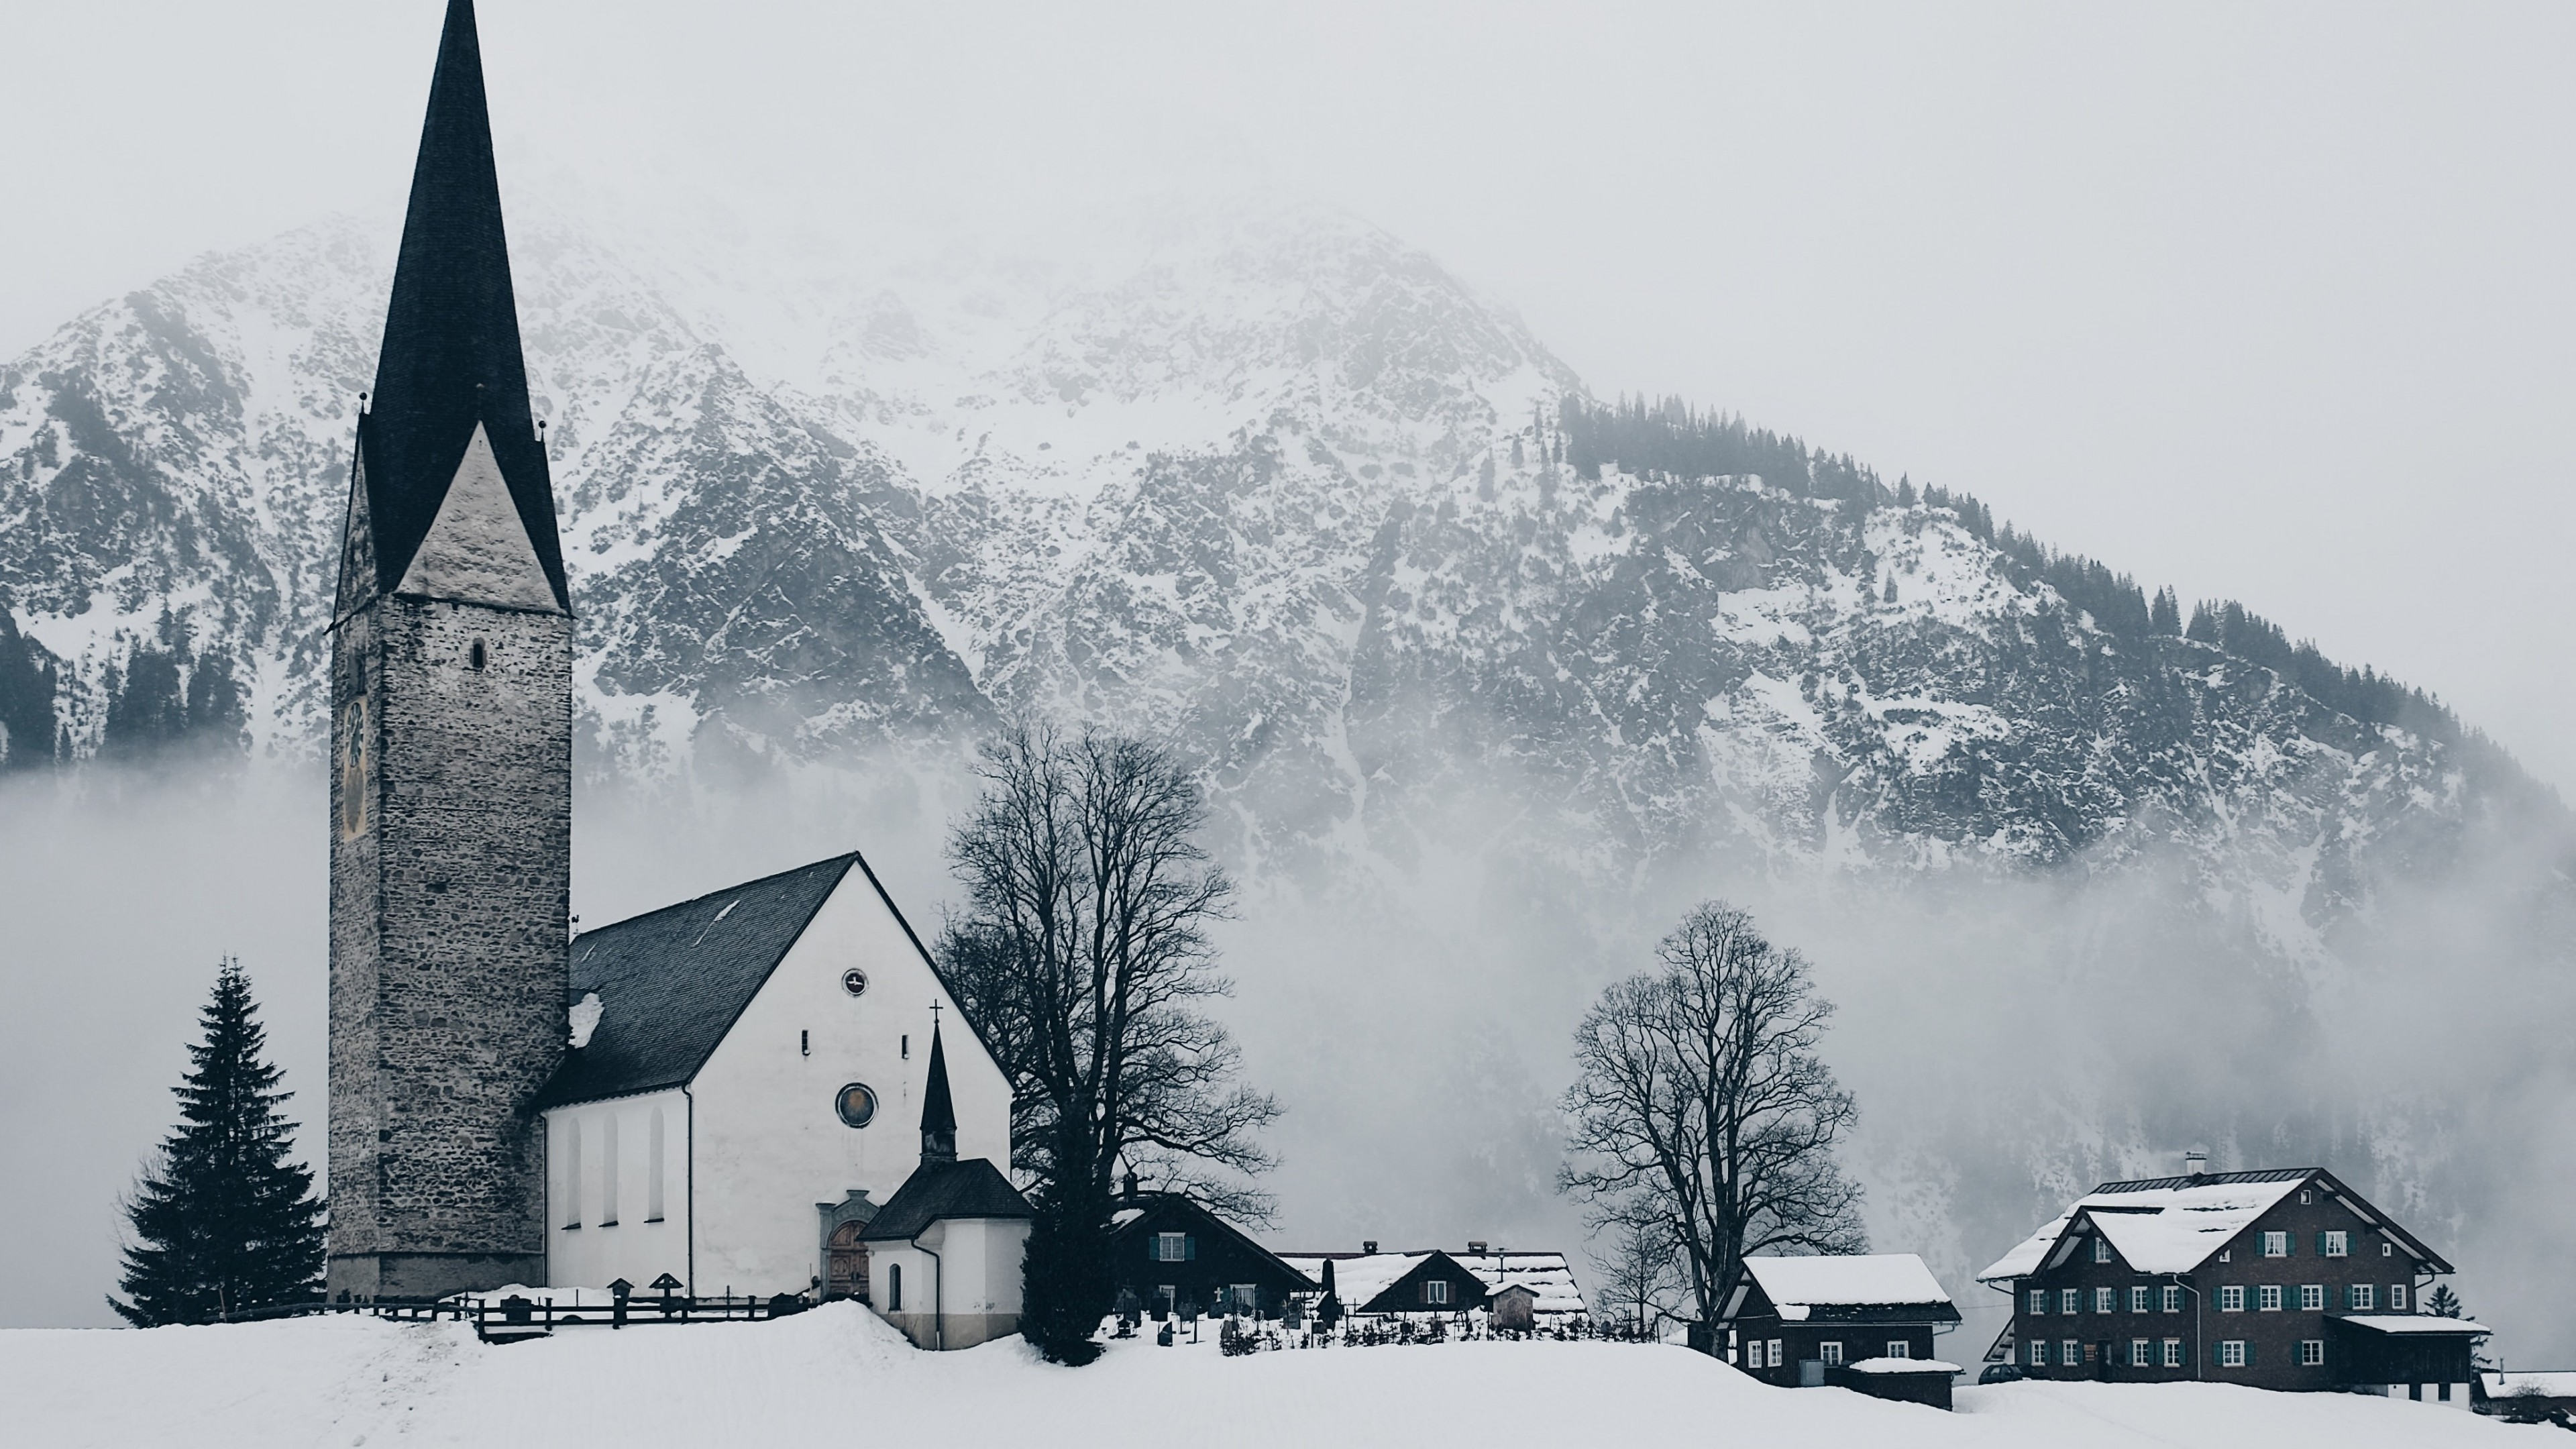
\includegraphics[width=5.5cm]{test_figure.jpg}
    \caption{This is a test figure}
    \label{fig:my_test_figure} % label用于在文档内容的其他位置使用\ref{fig:***}或\pageref{fig:***}来自动插入图表编号和所在页码
\end{figure}

Suspendisse volutpat fringilla lobortis. See figure \ref{fig:my_test_figure} on page \pageref{fig:my_test_figure}. Morbi ut pulvinar mauris. Aenean malesuada eu risus id mattis. Sed porta at diam vitae tincidunt. Donec laoreet justo eu eros commodo volutpat. 

% 插入表格(可以使用工具直接生成表格代码:https://www.tablesgenerator.com/)
\begin{table}[h]
    \centering
    \begin{tabular}{c|lc} % 这里是表格的内容,第二个括号内的参数用于设置表格的栏数、垂直格线样式、每栏的文字对齐方式(l c r)
         a & 1 & A \\ % 表格内每行的内容,以&符号作为每列之间的区分,以\\作为整行的结尾
         \hline % 插入水平格线
         b & 2 & B \\
         c & 3 & C 
    \end{tabular}
    \caption{This is a test table}
    \label{tab:my_test_table}
\end{table}

Vivamus eu nisl odio. Praesent vel scelerisque nisi. Nunc bibendum ullamcorper gravida. Suspendisse varius sapien in risus semper volutpat. Curabitur maximus convallis dui, vel pretium arcu euismod at. In at turpis dapibus, tincidunt orci sit amet, tempus leo. Etiam mattis mollis massa id auctor. Mauris tristique odio in mollis suscipit. In dignissim mollis pharetra. 

% 插入公式
% 与正文一起排版 - 在左右两端使用$符号来包裹公式内容,以表示这里有一个公式
Morbi id blandit arcu. Maecenas rhoncus scelerisque ex non tempor. Nulla facilisi. Nullam lobortis malesuada orci, bibendum interdum tortor pretium malesuada. $x^2 + y^2 = z^2$. Integer ut rhoncus diam. 

% 公式单独成一段且居中对齐 - 使用\[ 和 \] 把单独成行的公式套起来
\[
c^2 = a^2 + b^2
\]
% - 根号\sqrt{}
\[
c = \sqrt{a^2 + b^2}
\]
% - 分号\frac{分子}{分母},乘号\times
\[
2c = \frac{4 \times \sqrt{a^2 + b^2}}{2}
\]
% - 求和符号\sum_{下}^{上}{算式},下标用下划线x_i,上标用上尖x^2
\[
a = \sum_{i = 1}^{5}{\sqrt{x_i + b^2}}
\]



Suspendisse nibh mi, laoreet a molestie eget, condimentum in nisl. Maecenas lacinia metus feugiat, volutpat erat tincidunt, tincidunt lorem. Morbi aliquam commodo ante, ut molestie magna eleifend sit amet. Duis volutpat bibendum quam, lacinia blandit diam fermentum non. Nulla posuere, mi vel venenatis ultrices, quam eros porttitor nisl, quis euismod dolor lectus eu enim. Vivamus iaculis ex enim, non eleifend neque commodo ac. Donec mattis facilisis bibendum. Aenean id enim venenatis, convallis velit a, convallis mi. Proin dapibus eget tortor vel interdum. Sed volutpat ipsum at orci venenatis, eu tristique nisl posuere. Quisque luctus varius sapien at dignissim.

Sed purus urna, dignissim vitae commodo ut, finibus quis urna. Nam sollicitudin risus nibh, sed euismod metus varius ac. Quisque a tortor eget risus vestibulum consequat ullamcorper in dui. Phasellus at finibus ante, eu placerat augue. Donec volutpat turpis sed ex ultrices ornare. Fusce ipsum lorem, facilisis vel velit nec, commodo varius lectus. Donec viverra eget tortor nec sodales.\cite{xiang2022delightlcd} Nullam tempus nibh imperdiet felis dictum, eget maximus magna eleifend. \cite{zhang2022fine}
\section{第二章}
\section{第三章}

% 新建一个空白页插入参考文献列表,在正文中使用\cite{} - 此处只会列出真的在正文中使用\cite{}引用过的文献,所以可能不会完整列出.bib文件中的所有文献
\pagebreak
\bibliography{my_references}
\bibliographystyle{apacite}
\end{document}
